%%%%%%%%%%%%%%%%%%%%%%%%%%%%%%%%%%%%%%%%%%%%%%%%%%%%%%%%%%%%%%%%%%%%%%
% How to use writeLaTeX: 
%
% You edit the source code here on the left, and the preview on the
% right shows you the result within a few seconds.
%
% Bookmark this page and share the URL with your co-authors. They can
% edit at the same time!
%
% You can upload figures, bibliographies, custom classes and
% styles using the files menu.
%
%%%%%%%%%%%%%%%%%%%%%%%%%%%%%%%%%%%%%%%%%%%%%%%%%%%%%%%%%%%%%%%%%%%%%%

\documentclass[12pt]{article}

\usepackage{sbc-template}

\usepackage{graphicx,url}
\usepackage{pythonhighlight}
\usepackage{subfigure}
\usepackage[brazil]{babel}
%\usepackage[brazil]{babel}   
\usepackage[utf8]{inputenc}  

     
\sloppy

\title{Uma abordagem por Colônia de Formigas na resolução do Problema do Caixeiro Viajante}

\author{Rodrigo José Zonzin Esteves\inst{1}, Davi Silva Kunsch\inst{1}}


\address{Curso de Ciência da Computação \\ Departamento de Computação -- Universidade Federal de São João del Rei
  (UFSJ)\\
}

\begin{document} 

\maketitle

\section{Introdução}
De acordo com \cite{diestel2017graph}, a Teoria dos Grafos é uma área da Matemática que estuda as relações ebtre elementoss de um conjunto discreto de objetos, os vértices e arestas. Sua importância se dá pela capacidade de modelar sistemas complexos e suas inter-relações através de conceitos como proximidade, alcançabilidade, adjacência, centralidade e fluxo. 

O Problema do Caixeiro Viajante (PCV) é um problema clássico da Computação, por ser intratável em tempo polinomial. Nesse sentido, Heurísticas e Inteligência Artificial, como algoritmos genéticos e colônias de formigas, podem ser utilizados para encontrar soluções aproximadas, sem comprometer a eficiência da solução e um tempo computacional viável. \cite{goldbarg2012grafos}

O presente trabalho apresenta a modelagem e a implementação de um sistema de Colonia de Formigas em um PCV, obtendo resultados consistentes em diferentes iterações e convergentes para um ótimo global. 


\section{Problema do Caixeiro Viajante}
O PCV é uma questão central na área da otimização combinatória, demandando a determinação, em um grafo ponderado $G = (V, E)$, onde $V = \{v_1,..., v_n\}$ representa o conjunto de vértices e $E = \{e_1,..., e_m\}$ o conjunto de arestas, de um ciclo hamiltoniano que minimize o custo total percorrido. A identificação de um ciclo hamiltoniano de custo mínimo e máximo em um grafo sem propriedades distintivas é categorizado como um problema NP-Difícil. 

 Em Teoria da Complexidade, caracteriza-se NP-Dificil uma classe de problemas que são, de modo informal, "ao menos tão complexos quanto os problemas mais complexos em NP". Tal categoria de problemas suscita um interesse particular na Computação, exigindo estratégias e algoritmos sofisticados para sua resolução.
 
\section{Colônia de Formigas}
A heurística bioinspirada da Colônia de Formigas é uma das técnicas para contornar problemas Np-Dificeis  na resolução de problemas de otimização, fundamentado na simulação do comportamento cooperativo e adaptativo de formigas. Este princípio se baseia na cooperação de agentes individuais para solucionar desafios complexos por meio de comunicações simplificadas e na utilização de um mecanismo de rastreamento químico conhecido como feromônio.

A dinâmica fundamental desse método está no deslocamento das formigas, onde, ao percorrerem determinados caminhos, deixam para trás uma quantidade de feromônio, que influenciará a escolha de outra formigas. A deposição desse composto é essencial, servindo como um meio de comunicação entre as formigas, permitindo-lhes indicar rotas preferenciais e, consequentemente, cooperar na descoberta de soluções mais otimizadas.

Ao considerar um grupo de $m$ formigas, cada uma iniciando em uma cidade específica, presume-se que a presença conjunta desses agentes resultará na contribuição coletiva para a distribuição do feromônio. Outro pressuposto  é que trajetos vantajosos serão utilizados por múltiplas formigas, gerando um acúmulo maior de feromônio nessas rotas, consequentemente influenciando as decisões futuras das formigas e reforçando a utilização daquela rota.

No âmbito computacional desse modelo, a aproximação é realizada considerando que as formigas depositam feromônio em cada arco de um grafo $G = (V, E, P, F)$, onde $P$ representa os pesos das arestas e $F$ a quantidade de feromônio depositada.  


\subsection{Passos para a implementação}
Seja o grafo não direcionado $G=(V, E, W, F)$, onde $W$ representa os pesos de $E$ e $F$ a quantidade de feromônios em cada $e \in E$. 

Inicialmente, devemos definir as constantes de distância e feromônio que influenciam a probabilidade de uma formiga escolher determinado caminho. 

$$\tau_{xy} = \frac{1}{d_{xy}}, \forall xy \in E$$
$$\eta_{xy} = 0.1$$

Podemos então calcular a probabilidade de que uma formiga $k$ escolha o caminho $xy$ analisando o seguinte aspecto: quanto mais feromônio, maior deve ser a probabilidade de tomar o caminho e quanto maior a distância, menor. Temos, portanto, uma relação diretamente e inversamente proposcional. 

$$P^k_{xy} = \frac{[\tau_{xy}(t)]^\alpha [\eta_{xy}(t)]^\beta}{\sum_{l \in N^k_x} [\tau_{xy}]^\alpha[\eta_{xy}]^\beta}$$

Embora um caminho tenha uma probabilidade maior de ser escolhido, ele não deve ser sempre escolhido, pois o fenômeno é estocástico. Para modelar essa característica, devemos tomar a seguinte abordagem: 

$$CaminhoEscolhido_{k} = choice(xy \cdot p(xy)), \forall xy \in  CaminhosPossivesis_{k}$$
Essa abordagem deve ser recursiva, normalizando a probabilidade e retirando o vértice escolhido a cada momento. 
Ao final, teremos um caminho escolhido pela formiga, representado por $sequencia(k)$


Para atualizarmos o feromônio em uma rota $xy$ qualquer, tomamos 

$$(1-\sigma)\tau_{xy} $$

$$\Delta \tau_{xy}^k = \frac{Q}{d_k}$$

$$\eta_{xy}' = \sum  \Delta \tau_{xy}^k, \forall k \in sequencia(k) $$

Após atualizar os novos $\eta_{xy}'$, devemos recalcular as probabilidades $P_{xy}^k$ até que a soma das distâncias percorridas pelas formigas ($\sum sequencia(k) \ \forall k$) tenha convergido ou atingido um número máximo de iterações.

$\alpha=$ influencia do feromônio, $\beta =$, Q =taxa de atualização do feromônio, $\sigma$ = coeficiente de evaporação do feromônio.

\section{Resultados}
A figura \ref{grafo} apresenta o grafo obtido no arquivo \textit{lau15\_dist.txt}, obtido de \cite{citiesdataset}, constituído de 15 vértices numerados de 1 a 15 e suas respectivas arestas.

Os parâmetros selecionados são apresentados na tabela \ref{parametros}:

\begin{table}[]
    \centering
    \begin{tabular}{cc}
         Parâmetro & Valor  \\
         \hline 
         $\alpha$ & 1\\
         $\beta$ & 5\\
         max\_iteracoes & 1000\\
         Q & 10 \\
         $\sigma$ & 0.05\\
         \hline
    \end{tabular}
    \caption{Parâmetros obtidos de \cite{antcolonytspvideo}}
    \label{parametros}
\end{table}

A figura \ref{ensaio1} apresenta o caminho obtido no primeiro ensaio do nosso algoritmo, tendo custo final de 395. De maneira similar, as figuras \ref{ensaio2} e \ref{ensaio3}  apresentam os resultados obtidos em outros 2 ensaios. Note que os custos calculados foram, respectivamente, 390 e 401. 

Nossa abordagem parece convergir para um custo ótimo entre 390 e 400. 
Para verificar o impacto do número de iterações, observamos o custo calculado ao longo de 90 iterações. O resultado obtido é apresentado pela figura \ref{convergencia}, onde podemos observar uma tendência de queda até um limiar de estabilização em torno de um custo igual a 380.
\begin{figure}[h!]
    \centering
    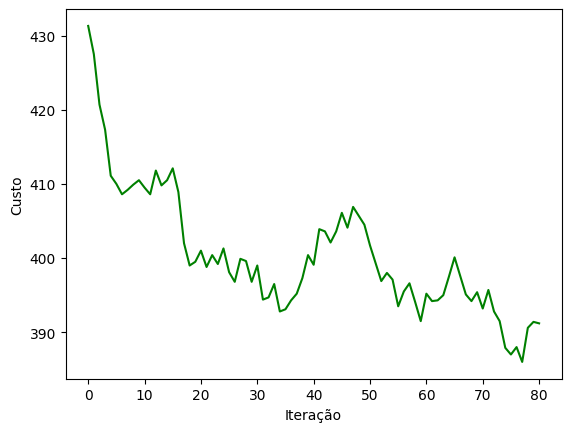
\includegraphics[width= 0.4\linewidth]{imgs/convergencia.png}
    \caption{Análise de Convergência}
    \label{convergencia}
\end{figure}
\newpage
Por completude, observamos as seguintes métricas: \textit{custo médio = 345, custo minimo observado = 402.35, custo máximo observado = 474, custo do último percentil = 378.9 e desvio padrão = 21.36 }
\begin{figure}[h!]
    \begin{minipage}{0.35\textwidth}
        \centering
        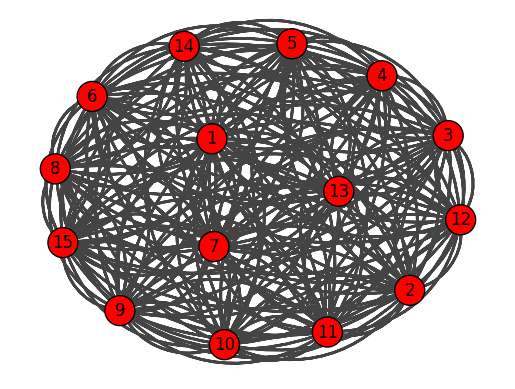
\includegraphics[width=\linewidth]{imgs/grafo_completo.png}
        \caption{Grafo}
        \label{grafo}
    \end{minipage}
    \hfill
    \begin{minipage}{0.4\textwidth}
        \centering
        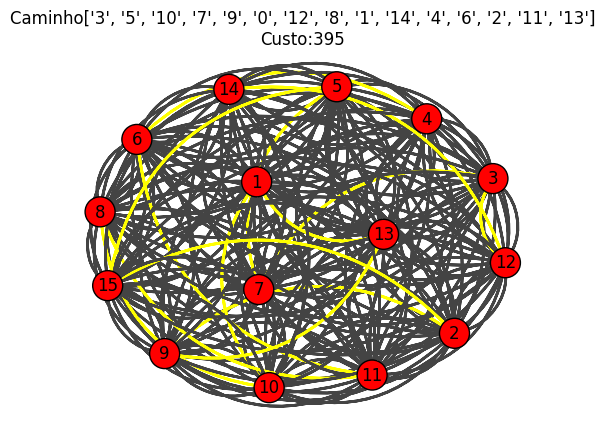
\includegraphics[width=\linewidth]{imgs/grafo_ensaio1.png}
        \caption{Ensaio 1}
        \label{ensaio1}
    \end{minipage}
    
    \begin{minipage}{0.4\textwidth}
        \centering
        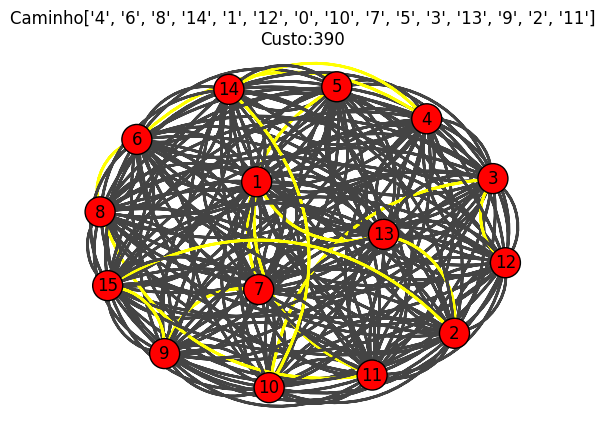
\includegraphics[width=\linewidth]{imgs/grafo_ensaio2.png}
        \caption{Ensaio 2}
        \label{ensaio2}
    \end{minipage}
    \hfill
    \begin{minipage}{0.4\textwidth}
        \centering
        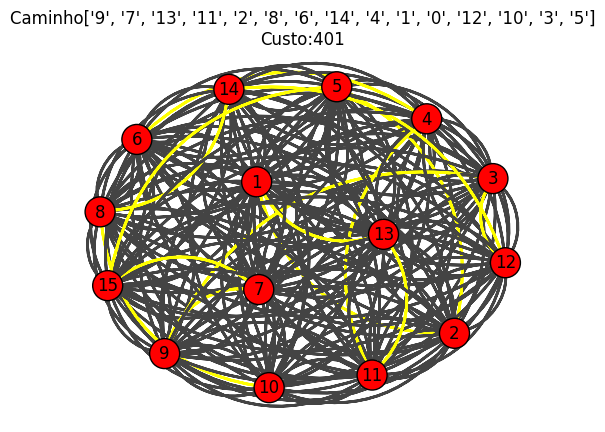
\includegraphics[width=\linewidth]{imgs/grafo_ensaio3.png}
        \caption{Ensaio 3}
        \label{ensaio3}
    \end{minipage}
    
    %\caption{Resultados obtidos}
    \label{resultados}
\end{figure}

\bibliographystyle{sbc}
\bibliography{sbc-template}


\end{document}
